\documentclass[11pt,aspectratio=169]{beamer}

\usepackage{slides}
\usepackage{soul}
\usepackage{pdfpc}
\usepackage{ebproof}
\usepackage{bigdelim}
\usepackage{booktabs}
\usepackage{listings}
\usepackage{tcolorbox}
\usepackage{tabularx}
\usepackage{tikz}
\usepackage{xspace}
\usepackage[T1]{fontenc}
\usepackage[utf8]{inputenc}
\usepackage[symbol]{footmisc}
\usepackage[noend]{algpseudocode}
\usepackage[
    backend    = biber,
    style      = alphabetic,
    giveninits = true,
    maxnames   = 16,
    minnames   = 16,
]{biblatex}

\addbibresource{./references.bib}

\usetikzlibrary{
    positioning,
    shapes.symbols,
    shadows,
    arrows,
    calc
}

\newcommand{\senc}{\text{senc}}
\newcommand{\msg}{\text{msg}}
\newcommand{\nonce}{\text{nonce}}
\newcommand{\KDF}{\text{KDF}}
\newcommand{\key}{\text{key}}

\newcommand{\Tamarin}[1]{\textsc{Tamarin}\xspace}

%% Print: [#1] -[#2]-> [#3]
\newcommand{\MSR}[3]{#1 -\hspace{-4pt}[\hspace{5pt} #2 \hspace{4pt}]\hspace{-4.6pt}\rightarrow #3}
%% Print: -[#1]->
\newcommand{\ActionFact}[1]{-\hspace{-4pt}[\hspace{5pt} #1 \hspace{4pt}]\hspace{-4.6pt}\rightarrow}
%% Print: ~
\newcommand{\tildelow}{\raisebox{0.5ex}{\texttildelow}}
%% Print: ^
\newcommand{\pow}{\textasciicircum{}}
%% Highlight text in overlay
\newcommand{\althl}[2][2]{\alt<#1>{\hl{#2}}{#2}}

%% Sticky notes to represent facts
\definecolor{StickyNoteYellow}{RGB}{241,239,161}
\definecolor{StickyNoteRed}{RGB}{255,167,169}
\definecolor{StickyNoteGreen}{RGB}{148,199,146}
\definecolor{StickyNoteBlue}{RGB}{167,229,241}
\NewDocumentCommand{\StickyNote}{O{StickyNoteYellow}O{1cm}m}{%
    \begin{tikzpicture}
        \node[
            drop shadow={
                shadow xshift = 2pt,
                shadow yshift = -4pt,
            },
            xslant = -0.1,
            yslant = 0.1,
            draw   = black,
            fill   = #1,
            text   = black,
        ] {\parbox[t][#2][c]{#2}{\centering#3}};
    \end{tikzpicture}
}

%% Colors for terms and facts
\definecolor{TermBlue}{HTML}{1C377D}
\definecolor{FactPurple}{HTML}{7C3655}

\newcommand{\term}[1]{\textcolor{TermBlue}{#1}}
\newcommand{\Term}[1]{\textcolor{TermBlue}{#1}}
\newcommand{\Fact}[1]{\textcolor{FactPurple}{#1}}

%% Other colors
\definecolor{AdversaryRed}{HTML}{DA3B26}

%% Listings
\lstset{escapeinside={(*@}{@*)}}
\lstset{numberstyle=\tiny}

\definecolor{TamarinBlue}{RGB}{42,0,255}
\definecolor{TamarinGreen}{RGB}{48,110,32}
\definecolor{TamarinPurple}{RGB}{175,36,67}

\lstdefinestyle{tamarin}{
    basicstyle    = \linespread{0.75}\footnotesize\ttfamily,
    extendedchars = true,
    tabsize       = 2,
    columns       = fixed,
    numbers       = none,
    breaklines    = true,
    literate      = {~}{{\raisebox{0.5ex}{\texttildelow}}}{1},
    morekeywords  = {theory, builtins, restriction, equations, functions, rule,
                     let, in, lemma, All, Ex, not, predicates, begin, end},
    keywordstyle  = \color{TamarinPurple},
    morecomment   = [l]{//},
    morecomment   = [s]{/*}{*/},
    commentstyle  = \color{TamarinGreen},
    xleftmargin   = 0mm,
    upquote       = true,
    morestring    = *[b]",
    showstringspaces = false
}

\lstdefinestyle{tactic}{
    basicstyle    = \linespread{0.75}\footnotesize\ttfamily,
    extendedchars = true,
    tabsize       = 2,
    columns       = fixed,
    numbers       = none,
    breaklines    = true,
    literate      = {~}{{\raisebox{0.5ex}{\texttildelow}}}{1},
    alsoletter    = :,
    morekeywords  = {tactic:, presort:, prio:, deprio:},
    keywordstyle  = \color{TamarinPurple},
    morecomment   = [l]{//},
    morecomment   = [s]{/*}{*/},
    commentstyle  = \color{TamarinGreen},
    xleftmargin   = 0mm,
    upquote       = true,
    morestring    = *[b]",
}

\lstdefinestyle{oracle}{
    basicstyle    = \linespread{0.75}\footnotesize\ttfamily,
    extendedchars = true,
    tabsize       = 2,
    columns       = fixed,
    numbers       = none,
    breaklines    = true,
    literate      = {~}{{\raisebox{0.5ex}{\texttildelow}}}{1},
    morecomment   = [l]{\#},
    morekeywords  = {import, for, in, if, elif},
    keywordstyle  = \color{TamarinPurple},
    commentstyle  = \color{TamarinGreen},
    xleftmargin   = 0mm,
    upquote       = true,
}

\definecolor{ProVerifGreen}{RGB}{48,110,32}
\definecolor{ProVerifBlue}{RGB}{64,112,161}

\lstdefinestyle{proverif}{
    basicstyle    = \linespread{0.75}\footnotesize\ttfamily,
    extendedchars = true,
    tabsize       = 2,
    columns       = fixed,
    numbers       = none,
    breaklines    = true,
    literate      = {~}{{\raisebox{0.5ex}{\texttildelow}}}{1},
    morecomment   = [s]{(*}{*)},
    commentstyle  = \color{ProVerifGreen},
    keywordstyle  = \color{ProVerifBlue},
    morekeywords  = {in, if, event, new, let, out},
    xleftmargin   = 0mm,
}

\definecolor{proofTreeBlue}{HTML}{2639B0}
\definecolor{proofTreeRed}{HTML}{921C12}

\lstdefinestyle{prooftree}{
    basicstyle    = \linespread{0.8}\footnotesize\fontfamily{pcr}\selectfont,
    extendedchars = true,
    tabsize       = 2,
    columns       = fixed,
    numbers       = left,
    breaklines    = true,
    literate      = {~}{{\raisebox{0.5ex}{\texttildelow}}}{1},
    keywords      = [1]{lemma, case, next, qed, by, end, Diff-Lemmas},
    keywordstyle  = [1]\color{black}\bfseries,
    keywords      = [2]{simplify, solve, sorry, contradiction, induction,
                        autoprove, rule-equivalence},
    keywordstyle  = [2]\color{proofTreeBlue}\bfseries,
    keywords      = [3]{@, \|, <, \^},
    keywordstyle  = [3]\color{proofTreeRed},
    alsoletter    = @\|<\^-,
    moredelim     = **[is][{\color{proofTreeBlue}}]{<<}{>>},
    xleftmargin   = 0mm,
    upquote       = true,
    morestring    = *[b]",
}

%% Color boxes
\definecolor{ColorBoxBlue}{HTML}{1C377D}
\tcbset{
    colback      = white,
    colframe     = black,
    fonttitle    = \bfseries,
    coltitle     = white,
    colbacktitle = ColorBoxBlue,
    boxrule      = 1pt
}

%% Vertical separator for frames
\newcommand<>{\vsep}{
    \begin{tikzpicture}[remember picture,overlay]%
        \draw[ultra thick]
            ($(current page.north west)+(8cm,0.5cm)$) to
            ($(current page.south west)+(8cm,-0.5cm)$)
        ;
    \end{tikzpicture}%
}

%% Horizontal separator for frames
\newcommand<>{\hsep}{
    \begin{tikzpicture}[remember picture,overlay]%
        \draw[ultra thick]
            ($(current page.north west)+(-0.5cm,-4.5cm)$) to
            ($(current page.north east)+(0.5cm,-4.5cm)$)
        ;
    \end{tikzpicture}%
}


\title{Formal Analysis of Real-World Security Protocols}
\subtitle{Lecture 6: Using Tamarin in Practice}
\date{\today}
\author{Aleksi Peltonen}
\institute{CISPA Helmholtz Center for Information Security}

\begin{document}
\maketitle

% ---------------------------------------------------------------------------- %
% Content
% ---------------------------------------------------------------------------- %

\begin{frame}[fragile]{This lecture}
    \tableofcontents
\end{frame}

% ---------------------------------------------------------------------------- %

\section{The Tamarin Prover}

% ---------------------------------------------------------------------------- %

\begin{frame}[fragile]{The Tamarin prover}
    \begin{columns}
        \begin{column}{0.6\textwidth}
            \begin{itemize}
                \item Originally developed at ETH Zurich by David Basin, 
                      Cas Cremers, Simon Meier, and Benedict Schmidt
                \item First version developed over 2-3 years, released in 2012
                \item Built on the experiences of previous tools (e.g., Scyther)
                \item Currently: four active maintainers and a large number of 
                      contributors
            \end{itemize}
        \end{column}
        \begin{column}{0.4\textwidth}
            \begin{figure}
                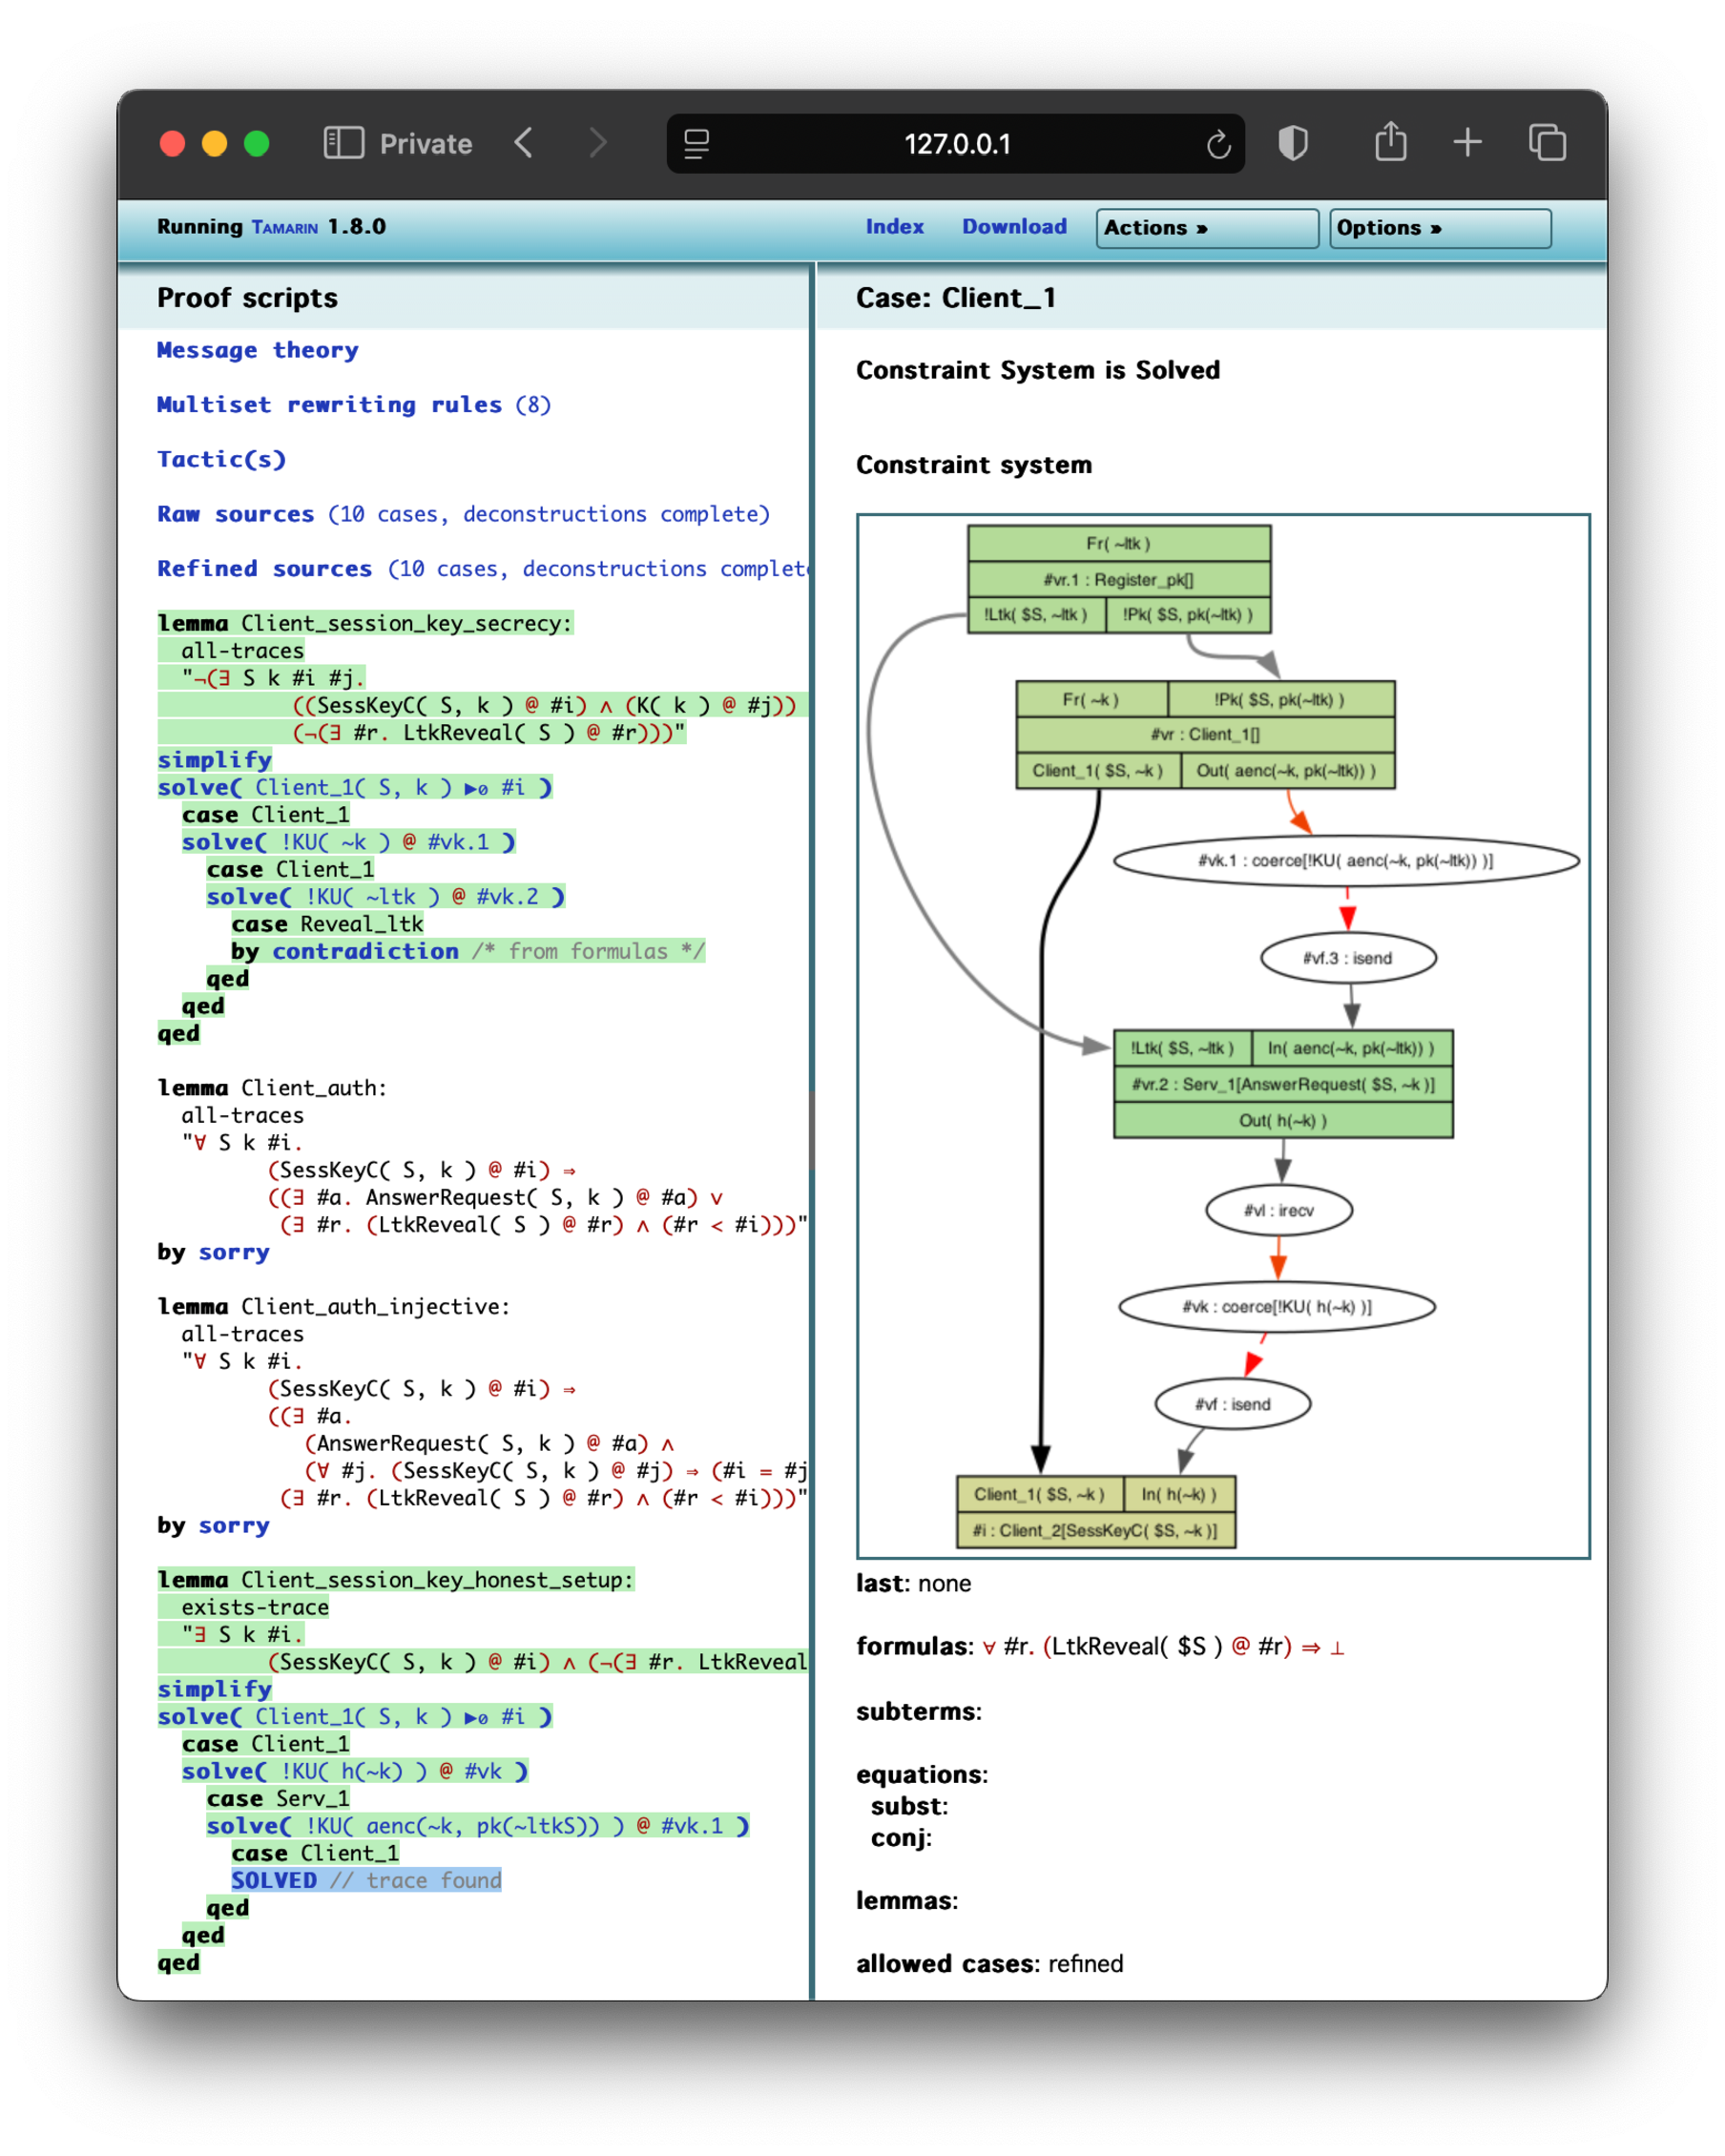
\includegraphics[width=.95\textwidth]
                    {./figures/lecture_0/tamarin_gui}
            \end{figure}
        \end{column}
    \end{columns}
    \begin{tikzpicture}[remember picture, overlay]
        \node[below left] at (current page.north east) {
            \frame{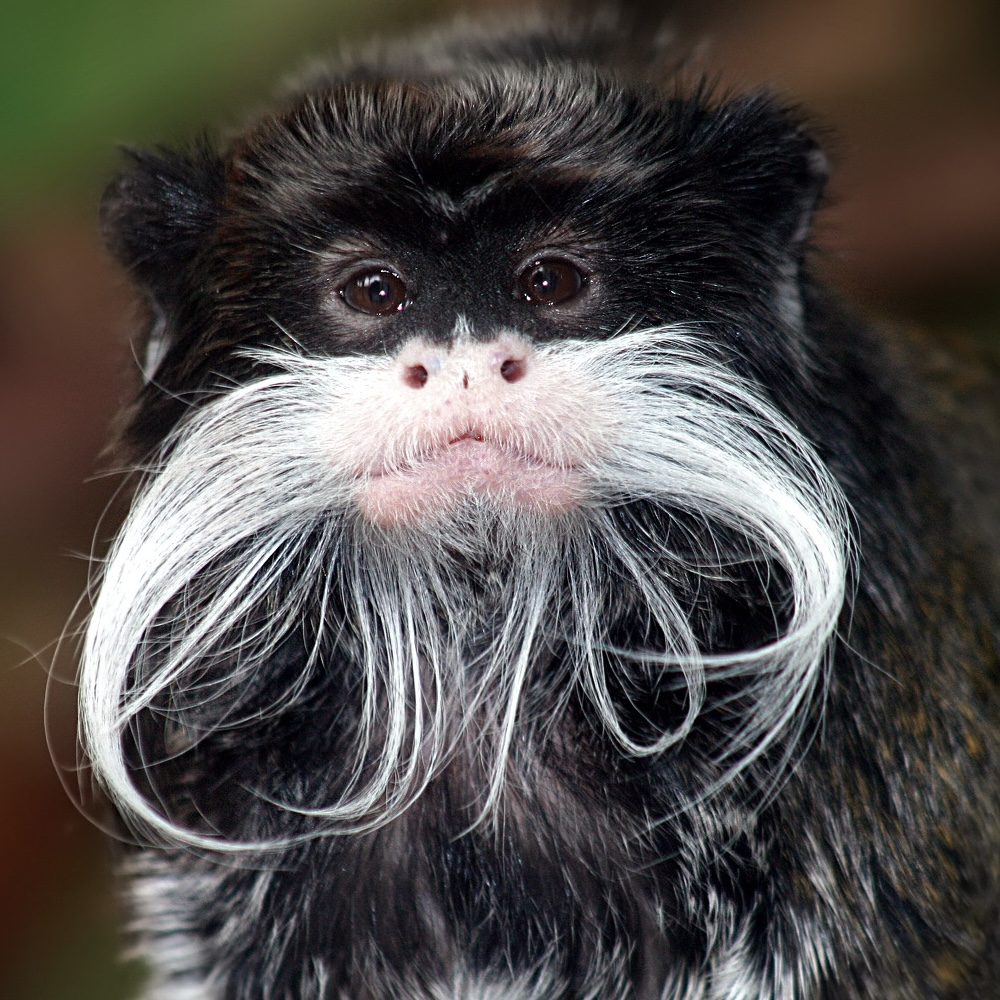
\includegraphics[width=0.08\textwidth]
                {./figures/lecture_0/tamarin_photo_small}}
            \frame{
\includegraphics[width=0.08\textwidth]
                {./figures/lecture_6/tamarin_logo_pixel}}
        };
    \end{tikzpicture}
    \setcounter{footnote}{0}
\end{frame}

\begin{frame}[fragile]{Resources}
    \begin{columns}
        \begin{column}{0.6\textwidth}
            Many additional resources available online
            \footnote[1,frame]{\url{https://tamarin-prover.com/}}:
            \begin{itemize}
                \item Extensive \textbf{user manual} with a focus on
                      ``\textit{explaining Tamarin's usage so that a new user 
                      can download, install, and use the system}.''
                \item Teaching material from summer schools, workshops, and 
                      tutorials
                \item Research papers on Tamarin, its theory, extensions, and 
                      case studies
            \end{itemize}
        \end{column}
        \begin{column}{0.4\textwidth}
            \begin{figure}
                \frame{\includegraphics[width=.8\textwidth]
                    {./figures/lecture_6/tamarin-manual}}
            \end{figure}
        \end{column}
    \end{columns}
\end{frame}

% ---------------------------------------------------------------------------- %

\section{Using Tamarin in Practice}

% ---------------------------------------------------------------------------- %

\begin{frame}[fragile]{Installing Tamarin}
    \begin{itemize}
        \item See instructions in the manual
        \item The easiest way to install Tamarin on macOS or Linux is to use 
              Homebrew (\verb|brew install tamarin-prover/tap/tamarin-prover|)
        \item Alternatively, you can also compile Tamarin from source
        \item For Windows, use Windows Subsystem for Linux (WSL)
    \end{itemize}
\end{frame}

\begin{frame}[fragile]{Getting started}
    \begin{columns}
        \begin{column}{0.5\textwidth}
            \begin{itemize}
                \item Input: *.spthy\\(
                      \textbf{s}ecurity \textbf{p}rotocol
                      \textbf{th}eor\textbf{y})
                \item Read Chapter 10 in the book for hints on getting started
            \end{itemize}
        \end{column}
        \begin{column}{0.5\textwidth}
            \vspace*{-.4cm}
            \lstinputlisting [
                style=tamarin,
                xleftmargin=.3cm,
            ] {./models/template.spthy}
        \end{column}
    \end{columns}
    \vsep
\end{frame}

\begin{frame}[fragile]{Writing models}
    \begin{itemize}
        \item Tamarin does not include an editor - use your favorite text 
              editor or IDE to write models
        \begin{itemize}
            \item Syntax highlighting (and other features) exists for e.g.,\\
                  VS Code, Vim, Sublime Text 3, GNU Emacs, and Notepad++
        \end{itemize}
        \item \textbf{Write readable models} by considering things like
        \begin{itemize}
            \item Indentation
            \item Consistent and self-explanatory naming convention
            \item \textbf{Comments} to explain the model
        \end{itemize}
    \end{itemize}
    \begin{onlyenv}
        \begin{columns}
            \begin{column}{0.49\textwidth}
                \begin{lstlisting}[
                    style = tamarin,
                    numbers = none,
                    gobble = 16,
                    xleftmargin = 2cm,
                    basicstyle = \linespread{0.75}\footnotesize\ttfamily,
                    literate = {~}{{\raisebox{0.5ex}{\texttildelow}}}{1},
                ]

                    rule r1:
                    [Fr(~a),Fr(~b)]
                    --[A(~a,~b)]->
                    [!B(~a,~b)]
                \end{lstlisting}
            \end{column}
            vs.
            \hspace*{1cm}
            \begin{column}{0.49\textwidth}
                \begin{lstlisting}[
                    style = tamarin,
                    numbers = none,
                    gobble = 16,
                ]
                    // Create new secret
                    rule derive_secret:
                      [ Fr(~id), Fr(~k) ]
                    --[ Secret(~id, ~k) ]->
                      [ !Secret(~id,~k) ]
                \end{lstlisting}
            \end{column}
        \end{columns}
    \end{onlyenv}
\end{frame}

\begin{frame}[fragile]{Command-line interface (CLI)}
    \begin{itemize}
        \item \textbf{Syntax:} \hspace*{.2cm}\verb|tamarin-prover *.spthy|
        \item Good for running large batches, bad for debugging
        \begin{itemize}
            \item Provides less feedback about potential problems
            \item Use when you think proof is working
        \end{itemize}
        \item Prove lemmas with the argument \verb|--prove[=LEMMA*]|
        \item Proofs can be exported with the argument \verb|--output=FILE|
        \item Supports Haskell's runtime system (RTS) parameters
              \verb|(+RTS -RTS)|\\e.g.,
              \verb|tamarin-prover model.spthy --prove=LEMMA +RTS -N4 -M4G -RTS|
        \item For a complete list of options, run \verb|tamarin-prover --help|
    \end{itemize}
\end{frame}

\begin{frame}[fragile]{CLI workflow}
    \begin{figure}
        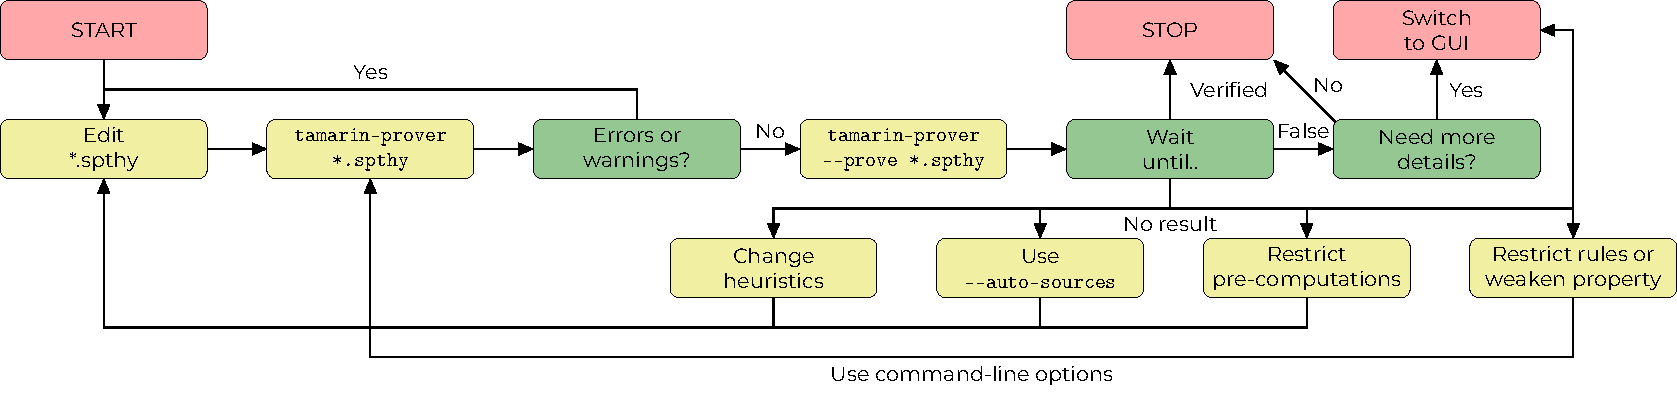
\includegraphics[width=\textwidth]{./figures/lecture_6/workflow_cli}
    \end{figure}
\end{frame}

\begin{frame}[fragile]{Graphical user interface (GUI)}
    \begin{itemize}
        \item \textbf{Syntax:}\hspace*{.2cm}
              \verb|tamarin-prover interactive [dir]|
        \item Loads all models in the given directory (e.g., \verb|.| for cwd) 
              and starts a server on port 3001
        \begin{itemize}
            \item Access server at \verb|http://127.0.0.1:3001|
            \item Possible to change port with the argument \verb|--port|
        \end{itemize}
        \item Possible to run remotely:
              \verb|ssh -L 3001:localhost:3001 SERVERNAME|
        \item No reloading; if you edit the model, you need to restart the 
              server
    \end{itemize}
\end{frame}

\begin{frame}[fragile]{GUI workflow}
    \begin{figure}
        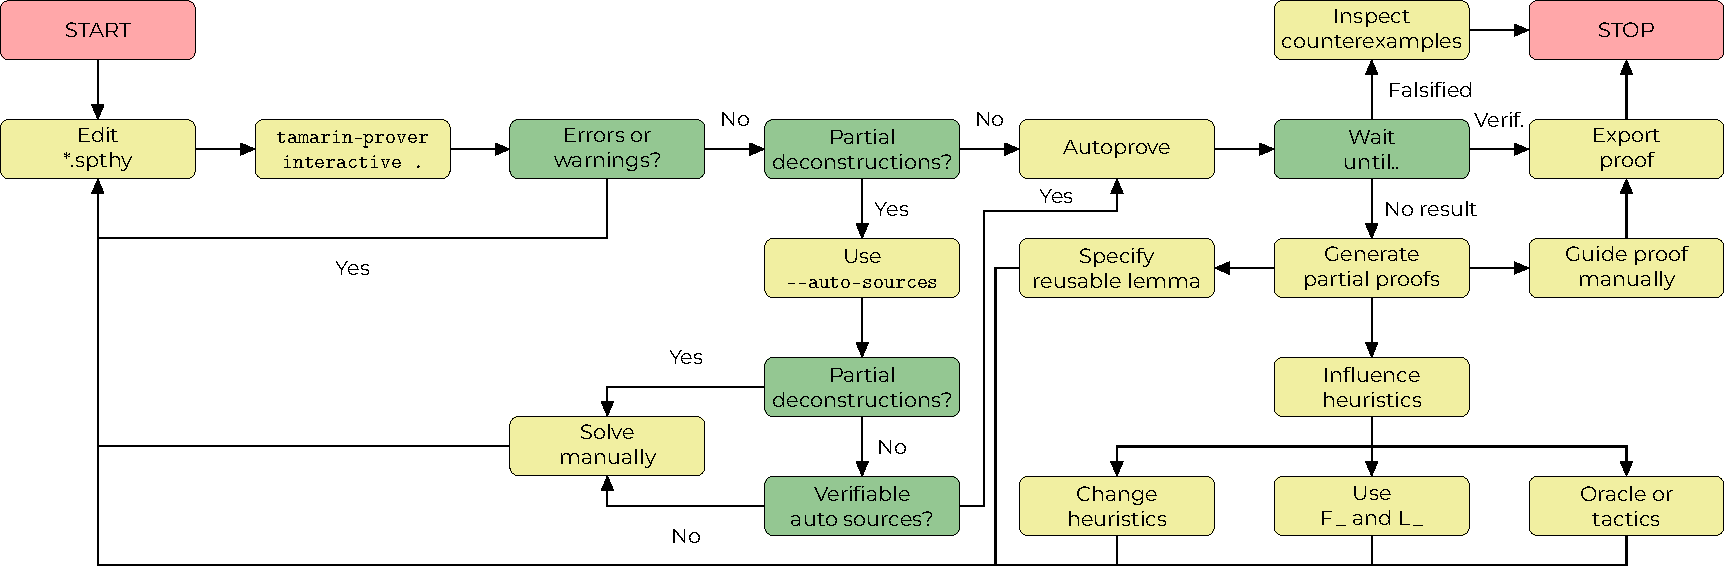
\includegraphics[width=\textwidth]{./figures/lecture_6/workflow_gui}
    \end{figure}
\end{frame}

\begin{frame}[fragile]{Syntactic correctness}
    \begin{columns}
        \begin{column}{0.6\textwidth}
            \begin{itemize}
                \item When loading a file, Tamarin will report \textbf{errors} 
                      and \textbf{wellformedness warnings}
                \item Most errors will not stop you from running the model, but 
                      may cause issues if not fixed
                \item Use the argument \verb|--quit-on-warning| to prevent 
                      Tamarin from proceeding if there are errors
                \item If you do not understand an error, see Chapter 11.4 in 
                      the book
            \end{itemize}
        \end{column}
        \begin{column}{0.4\textwidth}
            \begin{figure}
                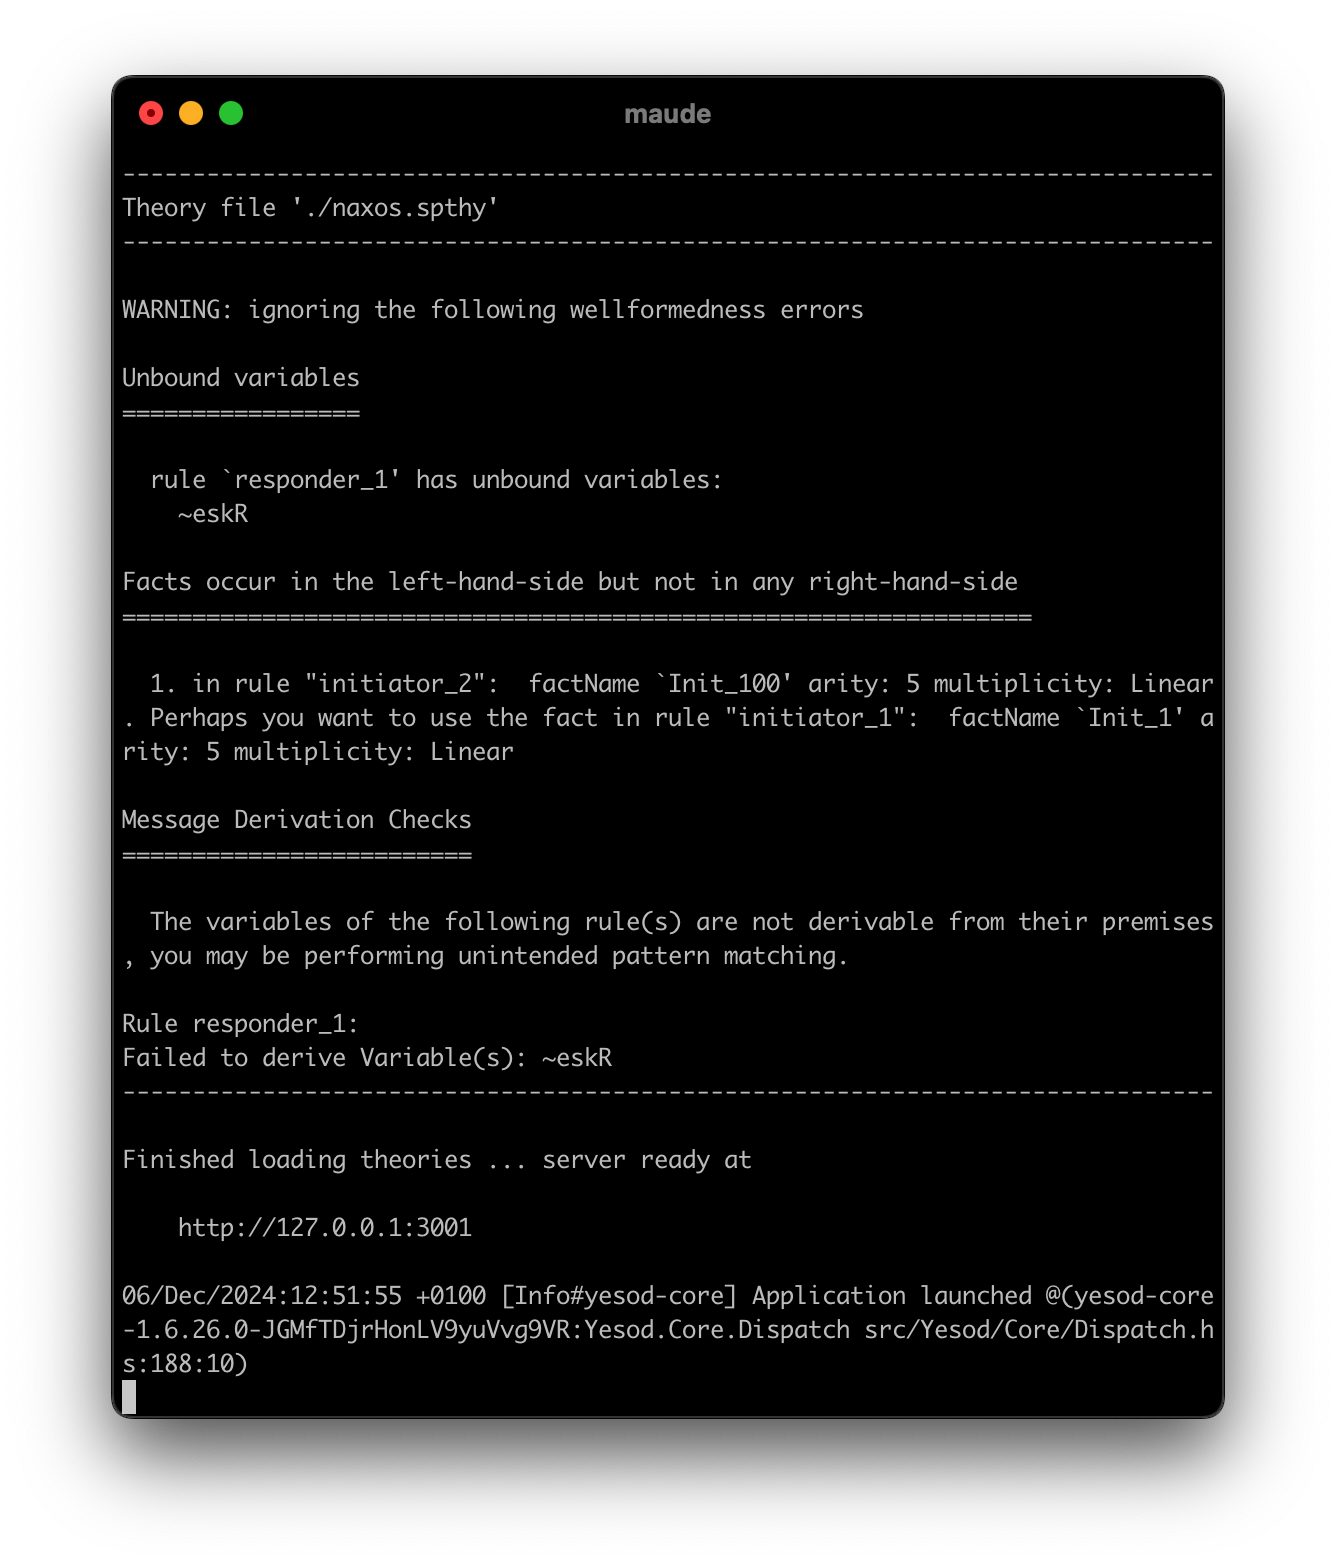
\includegraphics[width=\textwidth]
                    {./figures/lecture_6/wellformedness_conditions}
            \end{figure}
        \end{column}
    \end{columns}
\end{frame}

\begin{frame}[fragile]{Wellformedness checks}
    \begin{onlyenv}<1>
        \begin{itemize}
            \item No \texttt{Out} or \texttt{K} facts should appear in the 
                  premises of protocol rules and no \texttt{Fr}, \texttt{In}, 
                  or \texttt{K} facts should appear in the conclusions
            \item All action facts used in lemmas or restrictions should appear 
                  somewhere in the rules
            \item Facts must have the same arity everywhere, i.e., in all 
                  rules, lemmas, and restrictions
            \item \texttt{Fr}, \texttt{In}, \texttt{Out}, and \texttt{K} facts
                  must be of arity one
            \item \texttt{Fr} facts must be used with a variable of type 
                  message or type fresh
        \end{itemize}
    \end{onlyenv}
    \begin{onlyenv}<2>
        \begin{itemize}
            \item All lemmas must be guarded formulas
            \item All variables in the conclusions of a rule must appear in the 
                  premises, or be public variables
            \item The premises of a rule must not contain reducible function 
                  symbols such as decryption, XOR, etc
            \item The conclusions of a rule must not contain multiplication *
        \end{itemize}
        \begin{center}
            \textbf{Check the book for a complete lists of errors and how to 
                    fix them!}
        \end{center}
    \end{onlyenv}
\end{frame}

% ---------------------------------------------------------------------------- %

\section*{Example: NAXOS}

% ---------------------------------------------------------------------------- %

\begin{frame}[fragile,t]{NAXOS}
    \begin{figure}
        \includegraphics<1>[width=.5\textwidth]{./figures/lecture_6/naxos_1}%
        \includegraphics<2>[width=.5\textwidth]{./figures/lecture_6/naxos_2}%
    \end{figure}
\end{frame}

\begin{frame}[fragile]{Initialization}
    \begin{columns}
        \begin{column}{0.45\textwidth}
            \begin{figure}
                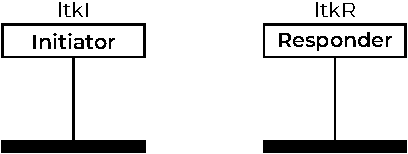
\includegraphics[width=.85\textwidth]
                    {./figures/lecture_6/naxos_pki}%
            \end{figure}
        \end{column}
        \begin{column}{0.55\textwidth}
            \lstinputlisting [
                style=tamarin,
                firstline=8,
                lastline=17,
                numbers=left,
                xleftmargin=.32cm,
            ] {./models/naxos.spthy}
        \end{column}
    \end{columns}
    \begin{tikzpicture}[remember picture,overlay]%
        \draw[ultra thick]
            ($(current page.north west)+(7cm,0.5cm)$) to
            ($(current page.south west)+(7cm,-0.5cm)$);
    \end{tikzpicture}%
\end{frame}

\begin{frame}[fragile]{Initiator model}
    \begin{columns}
        \begin{column}{0.45\textwidth}
            \begin{figure}
                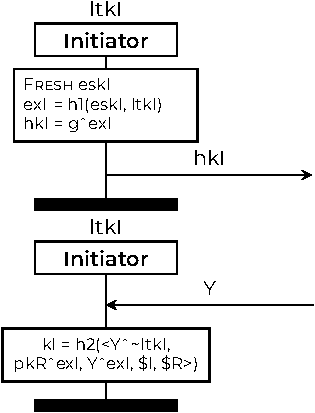
\includegraphics[width=.7\textwidth]
                    {./figures/lecture_6/naxos_init}%
            \end{figure}
        \end{column}
        \begin{column}{0.55\textwidth}
            \lstinputlisting [
                style=tamarin,
                firstline=19,
                lastline=28,
                numbers=left,
                xleftmargin=.32cm,
                firstnumber=11,
            ] {./models/naxos.spthy}%
            \lstinputlisting [
                style=tamarin,
                firstline=45,
                lastline=55,
                numbers=left,
                xleftmargin=.32cm,
                firstnumber=21,
            ] {./models/naxos.spthy}
        \end{column}
    \end{columns}
    \begin{tikzpicture}[remember picture,overlay]%
        \draw[ultra thick]
            ($(current page.north west)+(7cm,0.5cm)$) to
            ($(current page.south west)+(7cm,-0.5cm)$);
    \end{tikzpicture}%
\end{frame}

\begin{frame}[fragile]{Responder model}
    \begin{columns}
        \begin{column}{0.45\textwidth}
            \begin{figure}
                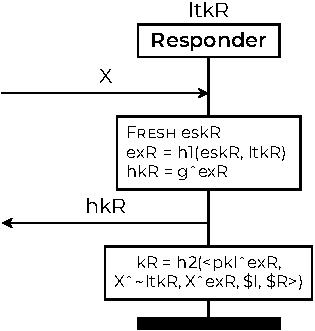
\includegraphics[width=.7\textwidth]
                    {./figures/lecture_6/naxos_resp}%
            \end{figure}
        \end{column}
        \begin{column}{0.55\textwidth}
            \lstinputlisting [
                style=tamarin,
                firstline=30,
                lastline=44,
                framextopmargin=1cm,
                numbers=left,
                xleftmargin=.32cm,
                firstnumber=32,
            ] {./models/naxos.spthy}
        \end{column}
    \end{columns}
    \begin{tikzpicture}[remember picture,overlay]%
        \draw[ultra thick]
            ($(current page.north west)+(7cm,0.5cm)$) to
            ($(current page.south west)+(7cm,-0.5cm)$);
    \end{tikzpicture}%
\end{frame}

% ---------------------------------------------------------------------------- %
% Reading Material
% ---------------------------------------------------------------------------- %
\begin{frame}[fragile]{Reading material}
    \textbf{Recommended reading}:
        ~\cite[Ch. 11]{tamarin-book},
    \begin{refsection}
        \nocite{tamarin-book}
        \printbibliography[heading=none]
    \end{refsection}
\end{frame}

\begin{frame}[fragile]{Reading material}
    \textbf{Additional reading}:
        ~\cite{cryptoeprint:2006/073},
        ~\cite{cryptoeprint:2008/376}
    \begin{refsection}
        \nocite{cryptoeprint:2006/073,cryptoeprint:2008/376}
        \printbibliography[heading=none]
    \end{refsection}
\end{frame}
% ---------------------------------------------------------------------------- %

\end{document}
